% The packages used here are just a sample. You may need others, and may not need some of these. It doesn't hurt to leave them in, unless they start to conflict with other packages you've added. Chapter 2 has example code for equations, figures, tables, citations, abbreviations, etc. If there are sections labeled 'optional' that you don't want, just comment them out. -jg

\documentclass[reqno,12pt,oneside]{report} % right-side equation numbering, 12 point font, print one-sided 
%\documentclass[reqno,12pt,twoside,openright]{report} % right-side equation numbering, 12 point font, print two-sided, Chapters start on odd pages. Rackham only accepts one-sided, so this is for personal printings.

\usepackage{rac}         % Use Rackham thesis style file
\usepackage{aas_macros}  % To allow the reading of ADS journal references in the bibliography
\usepackage[intlimits]{amsmath} % Puts the limits of integrals on top and bottom
\usepackage{amsxtra}     % Use various AMS packages
\usepackage{amsthm}
\usepackage{amssymb}
\usepackage{amsmath}
\usepackage{bm}% bold math
\usepackage{amsfonts}
\usepackage{graphicx}    % Add some packages for figures. Read epslatex.pdf on ctan.tug.org
\usepackage{rotating}
\usepackage{color}
\usepackage{epsfig}
\usepackage{subfigure}   % To make subfigures. Read subfigure.pdf on ctan.tug.org
\usepackage{verbatim}
\usepackage{natbib}      % Allows you to use BibTeX
\usepackage[printonlyused]{acronym} % For the List of Abbreviations. Read acronym.pdf on ctan.tug.org
\usepackage{setspace}    % Allows you to specify the line spacing
\doublespacing           % \onehalfspacing for 1.5 spacing, \doublespacing for 2.0 spacing.
\newcommand{\sun}{\ensuremath{\odot}} % sun symbol is \sun
\newcommand{\angstrom}{\mbox{\normalfont\AA}} %for angstrom symbol
%%%%%%%%%%%%%%%%%%%%%%%%%%%%%%%%%%%%%%%%%%%%%%%%%%%%%%%%%%%%%%%%%%%%%%%%%%%%%%%

% Various theorem environments. All of the following have the same numbering
% system as theorem.

\theoremstyle{plain}
\newtheorem{theorem}{Theorem}
\newtheorem{prop}[theorem]{Proposition}
\newtheorem{corollary}[theorem]{Corollary}
\newtheorem{lemma}[theorem]{Lemma}
\newtheorem{question}[theorem]{Question}
\newtheorem{conjecture}[theorem]{Conjecture}
\newtheorem{assumption}[theorem]{Assumption}

\theoremstyle{definition}
\newtheorem{definition}[theorem]{Definition}
\newtheorem{notation}[theorem]{Notation}
\newtheorem{condition}[theorem]{Condition}
\newtheorem{example}[theorem]{Example}
\newtheorem{introduction}[theorem]{Introduction}

\theoremstyle{remark}
\newtheorem{remark}[theorem]{Remark}
%%%%%%%%%%%%%%%%%%%%%%%%%%%%%%%%%%%%%%%%%%%%%%%%%%%%%%%%%%%%%%%%%%%%%%%%%%%%%%%

\numberwithin{theorem}{chapter}     % Numbers theorems "x.y" where x
                                    % is the section number, y is the
                                    % theorem number

%\renewcommand{\thetheorem}{\arabic{chapter}.\arabic{theorem}}

%\makeatletter                      % This sequence of commands will
%\let\c@equation\c@theorem          % incorporate equation numbering
%\makeatother                       % into the theorem numbering scheme

%\renewcommand{\theenumi}{(\roman{enumi})}

%%%%%%%%%%%%%%%%%%%%%%%%%%%%%%%%%%%%%%%%%%%%%%%%%%%%%%%%%%%%%%%%%%%%%%%%%%%%%%

% If printing two-sided, this makes sure that any blank page at the 
% end of a chapter will not have a page number. 
\makeatletter
\def\cleardoublepage{\clearpage\if@twoside \ifodd\c@page\else
\hbox{}
\thispagestyle{empty}
\newpage
\if@twocolumn\hbox{}\newpage\fi\fi\fi}
\makeatother 

%%%%%%%%%%%%%%%%%%%%%%%%%%%%%%%%%%%%%%%%%%%%%%%%%%%%%%%%%%%%%%%%%%%%%%%%%%%%%%

%This command creates a box marked ``To Do'' around text.
%To use type \todo{  insert text here  }.

\newcommand{\todo}[1]{\vspace{5 mm}\par \noindent
\marginpar{\textsc{To Do}}
\framebox{\begin{minipage}[c]{0.95 \textwidth}
\tt\begin{center} #1 \end{center}\end{minipage}}\vspace{5 mm}\par}

%%%%%%%%%%%%%%%%%%%%%%%%%%%%%%%%%%%%%%%%%%%%%%%%%%%%%%%%%%%%%%%%%%%%%%%%%%%%%%%
\DeclareUnicodeCharacter{2212}{-} %WARNING WARNING added by Mingfei
\overfullrule=0pt %WARNING WARNING added by Mingfei

\usepackage[]{graphicx}
\usepackage{lineno}
\usepackage[caption=false]{subfig}

\begin{document}

\bibliographystyle{agu04}    % Set the bibliography style. agu04, plain, alpha, etc. Original Rackham
%\bibliographystyle{alpha}    % Set the bibliography style. agu04, plain, alpha, elsarticle-num-names, etc.

% Title page as required by Rackham dissertation guidelines
\titlepage{Atomistic simulations of thermodynamics and kinetics related to advanced alloy processing}{Mingfei Zhang}{Doctor of Philosophy}
{Materials Science and Engineering}{2020}
{Assistant Professor Liang Qi, Chair\\
 Professor Amit Misra\\
 Associate Professor Emmanouil Kioupakis\\
 Professor Fei Gao}

% Begin the front matter as required by Rackham dissertation guidelines
\initializefrontsections

% Optional Frontispiece
%\frontispiece{\includegraphics[width=6in]{Intro/Happy} Find a cool picture to go here.}

% Optional, but recommended, Copyright page
%\copyrightpage{Your Name}

% Page numbering. If you don't include a frontispiece or copyright page, you'll need to change this for two-sided printing.
\makeatletter
\if@twoside \setcounter{page}{4} \else \setcounter{page}{1} \fi
\makeatother
 
% Optional Dedication page
\dedicationpage{Dedicated to my family.}

% Optional Acknowledgements page
\startacknowledgementspage
First and foremost, I would like to express my deepest gratitude to my advisor Prof. Liang Qi for his continuous guidance of my study, great patience, and immense knowledge. It is my honor to be the first student to join his research group. I am grateful for the open and inclusive collaboration culture he created across the group. I am fortunate to have Prof. Qi not only as a good mentor in academic research, but also as a good mentor in my life. Prof. Qi inspired me with his enthusiasm to science. The problem solving skills and attitude to others which I learned from him will guide me, no matter what I do in the future. I sincerely appreciate all he has done for me.

Besides, I would like to express my sincere thanks to Prof. Amit Misra, Prof. Emmanouil Kioupakis, and Prof. Fei Gao for serving on my thesis committee. The path to Ph.D. is long, rocky and confusing. Without their insightful suggestions, unlimited help, and generous encouragement, I could not have gone that far.

I also would like to thank my group mates: Chaoming Yang, Dr. Yong-Jie Hu, Aditya Sundar, Zhucong Xi, and Bin Bin for your help, your support, and many memorable moments. You guys are the best! I would like to thank other colleagues from U-M: Nocona Sanders, Dr. Erica Chen, and Dr. Cheng Zhang for their collaboration and discussion. I am also grateful to MSE Department for all the support. I also want to thank Dr. Louis Hector, Jr., Prof. L. Jay Guo, Dr. Jing-Yu Lao for their great collaboration. 

I am also grateful and feel lucky for funding supports provided by Materials Science and Engineering Department, Guardian Industry, General Motors, and National Science Foundation Grant Opportunities for Academic Liaison with Industry (GOALI) program. I thank computational resources provided by University of Michigan HPC Great Lakes, Extreme Science and Engineering Discovery Environment (XSEDE),  National Energy Research Scientific Computing Center (NERSC).

I would like to thank my dearest friends: Ruiming Lu, Dandan Wang, Patrick (Peng) Sun, and Judy (Xin-Yi) Song.

At last, I would like to thank my family. I would like to thank my parents for their support, understanding and love. And I would like to thank my beautiful wife Yan Zhang for her love, company and tolerance.
\label{Acknowledgements}

% Optional Preface page
%\startprefacepage
%\input{Preface}
%\label{Preface}

% Table of contents, list of figures, etc.
\tableofcontents     % Required
\listoffigures       % Required if there is more than one figure
\listoftables        % Required if there is more than one table
%\listofmaps          % Required if there is more than one map
\listofappendices    % Required if there is more than one appendix
\listofabbreviations % Optional. Abbreviations should be stored in a file named abbr.tex

% Optional in-dissertation Abstract Page
\startabstractpage
{Atomistic simulations of thermodynamics and kinetics related to advanced alloy processing}{Mingfei Zhang}{Chair: Liang Qi}
In my dissertation, the thermodynamic driving forces and kinetics of critical reaction steps during advanced alloy processing are studied systematically by theoretical models and simulation tools at the atomistic scale. These efforts include improving the Ag thin-film quality during sputtering, discovering a build-in corrosion-resistant mechanism for cast Mg alloys, and slowing down cluster nucleation and growth in Al solid solution alloys during natural aging to avoid costly hot stamping procedures. First, the thermodynamic driving force of H adsorption on anion-terminated (000$\overline{1}$) surfaces of pure and doped wurtzite ZnO as dielectric substrates are investigated under varying H surface coverage conditions. Understanding of these H adsorption mechanisms provides a general way to design substrate surfaces with desired binding strengths for the Ag thin-film. Second, \acf{GCMC} simulations are conducted to simulate the deposition "kinetics" of Ag thin film on substrates, which can be constructed based on the structures and properties of H-adsorbed ZnO (000$\overline{1}$) surfaces. The results demonstrate the reason why ZnO is the most suitable substrate for Ag thin film deposition and the mechanism to achieve thinner continuous Ag films by adding "anchor'' sites on the substrate surface. We use first-principles calculations to search for potential dopant elements as good "anchor'' sites on ZnO substrates and other dopants to stabilize the Ag grain boundaries to improve the polycrystalline Ag thin-film during heat treatment. Third, the \acf{HER} as the cathodic reaction on surfaces of the second-phase transition-metal (Fe) particles can speed up the corrosion of cast Mg metals and alloy. Thus, thermodynamic criteria to slow down the HER are used for high-throughput first-principles computations to search alloying elements that can reduce HER rate to achieve build-in corrosion resistance for cast Mg alloys. Our first-principles search goes across the periodic table and discovers six p-block elements that can increase the corrosion resistance for Mg, consistent with the available experimental results. Fourth, \acf{kMC} simulations are performed to study the early transition behavior from a supersaturated solid solution to \acf{GP} zone of Al 7000 series alloys at room temperature (so-called natural aging), which is critical for their thermal-mechanical processing in automobile manufacturing. Our kMC method include a \acf{NN} model trained by thousands of \ac{DFT} calculations to accurately predict vacancy migration barriers in Al-Mg-Zn-based alloys. Besides, advanced modeling approaches like \acf{LRU} cache and \acf{LSKMC} are also implemented to speed up the kMC simulations in order to directly study the natural aging of Al alloys in the realistic time scales.
\label{Abstract}

\startthechapters 
% The individual files for each of the chapters are put here.
% Save each chapter of your thesis to a seperate tex file
% and then use the \input command to include this file in your
% thesis.  For instance you can save a file to "intro.tex" and 
% then type \input{intro}. 

 \chapter{Introduction}
 \label{chap:Intro}
 This is an empty introduction for now. This is an empty introduction for now. This is an empty introduction for now. This is an empty introduction for now. This is an empty introduction for now. This is an empty introduction for now. This is an empty introduction for now. This is an empty introduction for now. This is an empty introduction for now. This is an empty introduction for now. This is an empty introduction for now. This is an empty introduction for now. This is an empty introduction for now. This is an empty introduction for now. This is an empty introduction for now. This is an empty introduction for now. This is an empty introduction for now. This is an empty introduction for now. This is an empty introduction for now. This is an empty introduction for now. This is an empty introduction for now. This is an empty introduction for now. This is an empty introduction for now. This is an empty introduction for now. This is an empty introduction for now. This is an empty introduction for now. This is an empty introduction for now. This is an empty introduction for now. This is an empty introduction for now. This is an empty introduction for now.

 \chapter{Methods}
 \label{chap:Methods}
 \section{Density Functional Theory}
\label{Chap:Mech:DFT}

In order to investigate interactions between hydrogen atoms and free surfaces of metals or oxides, we need to study their electronic structures. On the other hand, an accurate diffusion barrier energy also relies on a accurate reaction pathway. These can be achieved by first-principles methods. The calculation of interactions between the positively charged nuclei and negatively charged electrons is considered to be a many-body problem combining kinetic energy, interactions between nuclei and electrons, and electron-electron interactions. In principle, a quantum mechanical solution to this many-body problem with $N$ electrons in an external potential $V_{ext}(r)$ generated by the nuclei can be obtained by solving the Schr\"{o}vdinger’s equation. Based on the Born-Oppenheimer approximation, the motion of nuclei and electrons can be considered separately. Besides, $V_{ext}(r)$ can be obtained by calculating the Coulomb interactions between the atomic nuclei and electrons. The time-independent, non-relativistic Schr\"{o}dinger's equation for an N-electrons system can be written as,
\begin{subequations}
\begin{align}
\hat{H}\Psi & = E\Psi \label{Chap:Meth:DFT:eq:shdr1} \\
(-\sum_i^N \frac{\hbar^2}{2m}\nabla_i^2 + \sum_i^N V_{ext}(r) + \frac{1}{2}\sum_{i \neq j}^N\frac{1}{|r_i - r_j|}) \Psi & = E \Psi \label{Chap:Meth:DFT:eq:shdr2}
\end{align}
\end{subequations}
where $E$ denotes the system energy, $\Psi$ is the many-body wave function of electrons in the system, $\hat{H}$ is the Hamiltonian operator, $N$ is the total number of electrons in the system, $m$ is the mass of a single electron, $r_i$ denotes the position of electron $i$.


The many-body system will result in many variables in the wave function ($3N$ degrees of freedom), hence making it very difficult to solve. Due to the complexity and costly computation of directly solving Equation \ref{Chap:Meth:DFT:eq:shdr2}, \acf{DFT} provides a simpler method to transfer the many-body electron problem to a single-body problem based on the density functional of electrons. \cite{wilson1984electron, kohn1965self} First, Hohenberg and Kohn proved that for any system of interacting electrons in an external potential $V_{ext}(r)$, the potential $V_{ext}(r)$ is determined uniquely by the ground state electron density $\rho_0(r)$, which means the Hamiltonian in Equation \ref{Chap:Meth:DFT:eq:shdr1} is solely determined by the ground state electron density $\rho_0(r)$. Second, the ground state energy of the system may be obtained variationally, such that the electron density $\rho(r)$ that can minimizes the total energy is the ground state density $\rho_0(r)$ exactly. In the Kohn-Sham system, the electron density $\rho(r)$ of $N$ electrons \cite{kohn1965self} is expressed as,
\begin{subequations}
\begin{align}
\rho(r) & = \sum_i^N {|\phi_i(r)|}^2 \label{Chap:Meth:DFT:eq:ks_rho}
\end{align}
\end{subequations}
where $\phi_i(r)$ is the Kohn-Sham orbital which is solved by using the Kohn-Sham Schr\"{o}vdingerr-like equation:
\begin{subequations}
\begin{align}
(H_{KS} - \epsilon_i) \Psi_i(r) & = 0 \label{Chap:Meth:DFT:eq:ks_1}
\end{align}
\end{subequations}
where $\Psi_i(r)$ is the eigenvector and $\epsilon_i$ is the corresponding eigenvalue or orbital energy for a non-interacting electron. $H_{KS}$ is the effective Kohn-Sham Hamiltonian defined as,
\begin{subequations}
\begin{align}
  H_{KS} & = -\frac{\hbar^2}{2m}\nabla_i^2 + V_{ext}(r) + V_{Hartree}(r) + V_{xc}(r) \label{Chap:Meth:DFT:eq:ks_H} \\ 
  \hfill
  V_{Hartree}(r) & = e^2\int \frac{\rho(r)}{|r - r'|} d^3r \label{Chap:Meth:DFT:eq:ks_Hartree}\\ 
  \hfill
  V_{xc}(r) & = \frac{\partial E_{xc}(\rho(r))}{\partial \rho(r)} \label{Chap:Meth:DFT:eq:ks_xc} 
\end{align}
\end{subequations}
In Equation \ref{Chap:Meth:DFT:eq:ks_H}, $V_{ext}(r)$ is still the potential accounting for the electron-nuclei interaction as Equation \ref{Chap:Meth:DFT:eq:shdr2}, $V_{Hartree}(r)$ is the Coulomb electron-electron interaction as defined in Equation \ref{Chap:Meth:DFT:eq:ks_Hartree}, $V_{xc}(r)$ is the exchange-correlation potential as obtained by Equation \ref{Chap:Meth:DFT:eq:ks_xc}, which accounts for the nonphysical self-interaction error, alongside with other effects. This term is unknown in the Kohn-Sham equation which is the reason why it is the derivative to its energy expression. However, approximation exists and depends only on the value of $\rho(r)$ at a coordinate in space where the functional is evaluated. This method is also known as the \acf{LDA}. \cite{perdew1981self} DFT results from \ac{LDA} approximations usually yield a good estimation of atomic geometries of studied system, but may overestimate the binding energies between different species. A better solution comes from \acf{GGA}. \cite{perdew1986density} The \ac{GGA} method is local but it also incorporates the effects of inhomogeneity by including the gradient of electron density at the same coordinate. \cite{ceperley1980ground} And \ac{GGA} method usually gives good estimations of the ground state energies, so it is widely used in surface calculations and transition states calculations. There are many different implementations of GGA have been developed: for examples, 1) PW91-GGA from Perdew and Wang (PW91-GGA) \cite{perdew1992accurate}, 2) PBE-GGA from Perdew, Burke and Ernzerhof (PBE) \cite{perdew1996generalized}, and 3) revised PBE-GGA for solids (PBEsol) \cite{perdew2008restoring}. Based on these approximate functionals for exchange-correlations, the Kohn-Sham Equation \ref{Chap:Meth:DFT:eq:ks_1} can be solved based on iterative methods.
\section{Grand Canonical Monte Carlo Simulation}
\label{Chap:Mech:GCMC}

\subsection{Grand Canonical Ensemble}

The canonical ensemble is a statistical ensemble that consists of $N$ atoms and is in thermodynamic equilibrium with a big reservoir. Energy transfer is allowed between the system and the big reservoir, but particle transfer is impermissible. The big reservoir can be described as a system with relatively large heat capacity, and its temperature $T$ remains constant in spite of any energy transfer. Grand canonical ensemble is a statistical ensemble that can exchange particles with a reservoir as an open system. Besides, the big reservoir can also act as an infinite heat resource allowing heat transfer as shown in Figure \ref{Chap:Meth:GCMC:fig1}. \cite{frenkel2001understanding} Therefore in the grand canonical ensemble, the number of atoms $N$ in the system can be changed and chemical potential of each element $\mu_i$, the volume of the system $V$ and temperature $T$ are fixed, hence this system is known as $\mu VT$ system.

\begingroup
\begin{figure}[!ht]
  \centering
  \subfigure{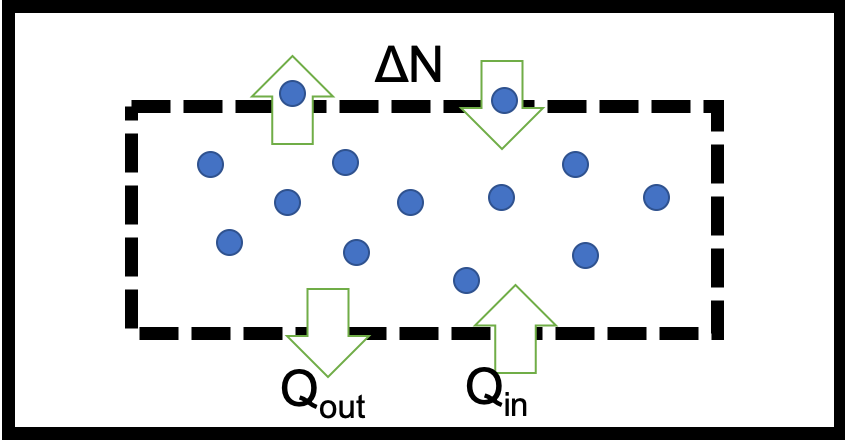
\includegraphics[width=0.45\linewidth]{Methods/plots/grand-canonical-ensemble.png}}
  \caption[Illustration plot of grand canonical ensemble.]{Illustration plot of grand canonical ensemble. Black line shows the universe. Black dashed line confines the ensemble. Blue solid circles are atoms in the system.}
  \label{Chap:Meth:GCMC:fig1}
\end{figure}
\endgroup

\subsection{Monte Carlo Methods}
\label{Chap:Mech:GCMC:MC}

\ac{MC} methods are a broad class of computational algorithms that rely on repeated random sampling to obtain numerical results for a problem that is difficult to solve in principle. The physics behind is to use randomness to solve problems that might be deterministic. They are often used in mathematical \cite{hubbard2009modeling} and physical \cite{bortz1975new} problems. In this thesis, \ac{MC} methods are used to do optimization for complex \ac{GB} structures in Chapter \ref{Chap:Ag/ZnO:GB}, thin-film morphology in Chapter \ref{chap:Ag/ZnO} and solving stochastic time evolution in Chapter \ref{chap:Al/Vac}. A general \ac{MC} algorithm involves: i) drawing a random number $u \in (0,1]$ and ii) accepting/rejecting event base on Boltzmann probability.

\subsection{Grand Canonical Monte Carlo Simulation}
\label{Chap:Mech:GCMC:GCMC}

\ac{GCMC} simulation combines the grand canonical ensemble with \ac{MC} simulations. Following grand canonical($\mu VT$) ensemble discussed above, the number of atoms $N$ in the ensemble can be changed, thus grants two types of events, inserting a new atom and deleting an existing atom. In addition to these two events, moving an atom to a different location is also considered in the event list. Therefore, the probability of accepting moving an existing atom is via \cite{frenkel2001understanding}:
\begin{align}
acc(s \rightarrow s') = \text{min}(1, exp(-\beta(U(s'^N) - U(s^N))
\label{Chap:Meth:eq:acc:move}
\end{align}
inserting a new atom:
\begin{align}
acc(N \rightarrow N+1) = \text{min}(1, \frac{V}{\wedge^3(N+1)}exp(\beta(\mu - U(N + 1) + U(N)))) \label{Chap:Meth:eq:acc:insert}
\end{align}
and removing an existing atom:
\begin{align}
acc(N \rightarrow N-1) = \text{min}(1, \frac{\wedge^3(N)}{V}exp(-\beta(\mu + U(N - 1) - U(N)))) \label{Chap:Meth:eq:acc:remove}
\end{align}
where, $\beta$ is the thermodynamic beta and $\wedge$ is the de Broglie wavelength. Additionally, \ac{MD} steps are usually combined together with \ac{GCMC} simulations to reduce the thermal instability or stress introduced by randomly inserting and moving atoms, as know as the hybird \ac{MC}/\ac{MD} method in Chap. 4.4 of Frenkel 2001 \cite{frenkel2001understanding}. Atomic structures in my thesis are generated by Atomeye, a high efficient visualization tool for millions of atoms. \cite{li2003atomeye}
\section{Kinetic Monte Carlo Simulation}
\label{chap:meth:KMC}

Many real reactions will take a long time, for example, hours, to happen, so the reaction kinetics are difficult to observe by only using \ac{DFT} calculations or \ac{MD}. As discussed in Section \ref{Chap:Mech:GCMC:MC}, \ac{MC} method is used here to help to solve stochastic time evolution in a much longer time scale. Much previous research used this method to simulate vacancy bulk diffusion, surface diffusion, and surface growth. \cite{frenkel2001understanding, leach2001molecular} A typical \ac{kMC} method is shown in Algorithm \ref{algo:kMC}.

\begin{figure}[htb]
\centering
\begin{minipage}{.7\linewidth}
\begin{algorithm}[H]
  \caption{Kinetic Monte Carlo Algorithm}\label{algo:kMC}
  \begin{algorithmic}[1]
    \State Start the simulation at time t = 0.
    \While {$t < t_{Max}$ Or $epoch < epoch_{Max}$}
        \State Build or update an event list for all the possible event i with rate $r_i$ in the system.
        \State Calculate the cumulative rate $R = \sum_{j=1}^N r_j$,
            where $N$ is the total number of events. 
        \State Calculate probability, $p_i$, of event i by normalizing $r_i$ by $R$.
        \State Generate two uniform random number $u, v \in (0, 1]$.
        \State Choose the event $i$ based on,
               $\sum_{k=1}^{i-1} p_k < u < \sum_{k=1}^{i} p_k$.
        \State Carry out the event $i$.
        \State Update the time with $t = t + \Delta t$,
            where $\Delta t$ is obtained via
            \begin{align}
                \Delta t = - \frac{\log{v}}{R_N}
            \label{Chap:Meth:eq:KMC:1}
            \end{align}
    \EndWhile
\end{algorithmic}
\end{algorithm}
\end{minipage}
\end{figure}

For a system of vacancy on-lattice diffusion in bulk materials, each event rate can be calculated from \ac{DFT} with \ac{NEB} method in principle. However, \ac{NEB} calculations are extremely time-consuming for simulating billions of steps for \ac{kMC}. And the relationship between diffusion barriers and energy differences are not linear for multi-component systems. Therefore, the \ac{NN} functional is trained based on \ac{DFT} calculations to predict diffusion barriers. Thus, we can build a multi-scale methodology, which combines \ac{DFT}, \ac{NN}, and \ac{kMC}, to study the thermodynamics and kinetics of the early nucleation stage of GP zone in Al alloys.
\section{Deep Learning and Neural Network}
\label{Chap:Mech:NN}

As previously mentioned in Chapter \ref{Chap:Mech:DFT}, \ac{DFT} calculations are accurate but also computationally costly. In order to solve the short time span of \ac{DFT} simulations, researchers fit \ac{DFT} results to classical force fields or empirical interatomic potentials, which are simpler analytical formulas or functional. Classical force fields or empirical interatomic potentials simplify the description of inter-atomic interactions by summing components of the short-ranged bonding\cite{jones1924determination}, angular\cite{justo1998interatomic}, dihedral\cite{cornell1995second}, and long-ranged Coulomb interaction\cite{liang2013classical}. Empirical potentials can be used in large-scale atomistic simulations with a reduced computational cost. Scientists and researchers have been constantly working on fitting more accurate empirical potentials to improve statistical sampling and accuracy of \ac{MD} and \ac{MC} simulations for the longer time domain. Due to the simplicity of analytical formulas and costly \ac{DFT} calculations, empirical potentials can only focus on a limited number of material properties of the fitted system. As the number of species included in the system increases, it is also more difficult to fit the desired empirical potential. Besides, empirical potentials are, in general, good at describing the interactions close to the equilibrium, but not very well at intermediate or transitional states. Therefore, to study the early nucleation stage of multi-component systems via vacancy diffusion, a more complex functional need to be used, which could be machine learning or \acf{NN} methods.

\begingroup
\begin{figure}[!ht]
  \centering
  \subfigure[]{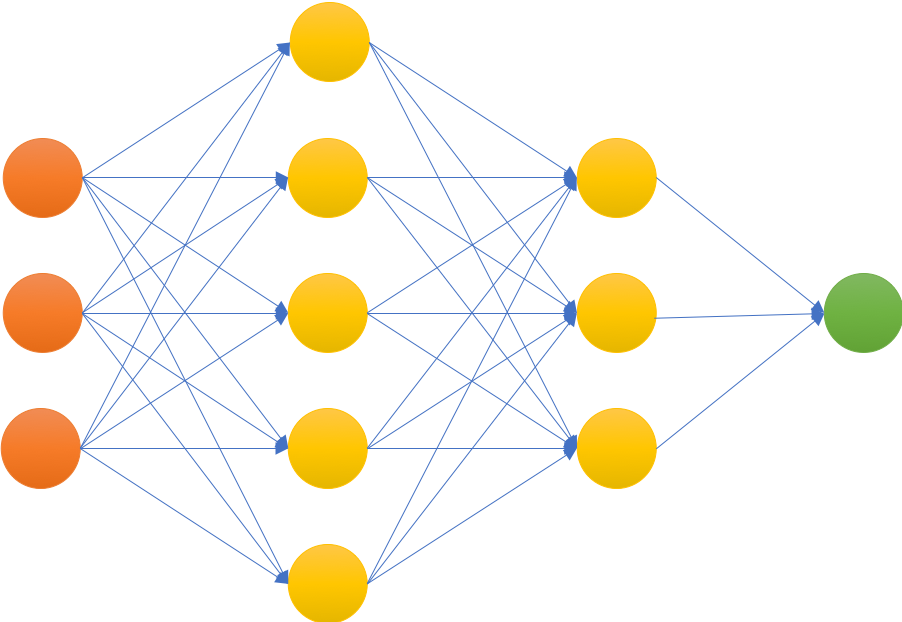
\includegraphics[width=0.9\linewidth]{Methods/plots/nn.png}}
  \caption[Illustration plot of a neural network.]{Illustration plot of a neural network. Orange, yellow, and green nodes indicate the input layer, hidden layers, and output, respectively.}
  \label{Chap:Meth:NN:fig1}
\end{figure}
\endgroup
Recently, machine learning methods have been widely used in materials science to construct the interatomic force fields in complex multi-component systems\cite{artrith2016implementation}, predict material properties\cite{hu2019local,hu2020predicting}.
Deep learning (or \ac{NN}) is a special category of machine learning models that uses a network of neurons, which are arranged in (fully/partially) interconnected layers. A \ac{NN} works similarly to the human brain’s neural connectivity, which will be activated under certain circumstances using various activation functions. \ac{NN}s are non-linear functions with parameters in different layers, called weights. Weights are optimizable through the back-propagation method of a cost function with respect to each weight. The input layer collects input patterns. The output layer has classifications or regression values to which input patterns are related. Hidden layers fine-tune the input weighting parameters until the \ac{NN}’s cost function is minimal. It is hypothesized that hidden layers extrapolate features in the input data that have predictive power about the outputs. In Figure \ref{Chap:Meth:NN:fig1}, a two-layer \ac{NN} is shown. Three orange nodes on the left indicate input nodes, which can be atom species encoding in the on-lattice bulk diffusion model. Yellow nodes in the middle are two layers of fully connected hidden layers. The green node on the right is the output layer, which can be the diffusion barrier. In practice, the neural network architecture will be much more complicated. Details of fitting diffusion barriers will be discussed in Chapter \ref{chap:Al/Vac}.
 
 \chapter{formatting reference chapter}
 \label{chap:format}
 \section{Introduction}
\label{Transport Intro}
For reference, some common equations and brief overviews of the three categories of particles will be given in this chapter. The Maxwell equations \eqref{Gauss}--\!\,\eqref{Ampere}, the continuity equation for charge density and current density \eqref{continuity}, the Lorentz force equation \eqref{Lorentz}, Newton's second law of motion \eqref{Newton2}, and the \ac{MHD} approximation of Ohm's Law \eqref{Ohm} are each useful for basic plasma physics. Thorough derivations for these and related equations can be found in several textbooks, including \citet{gombosi98} and \citet{jackson99}.

\begin{subequations}
 \begin{align}
  \nabla\cdot\mathbf{E}&=\frac{\rho_e}{\epsilon_0}&\quad\text{Gauss's Law}
  \label{Gauss}\\
  \nabla\times\mathbf{E}&=-\frac{\partial\mathbf{B}}{\partial t}&\quad\text{Faraday's law of induction}
  \label{Faraday}\\
  \nabla\cdot\mathbf{B}&=0&\quad\text{Gauss's law for magnetism}
  \label{Gauss m}\\
  \nabla\times\mathbf{B}&=\mu_0\mathbf{J}+\mu_0\epsilon_0\frac{\partial\mathbf{E}}{\partial t}&\quad\text{Amp\`{e}re's law}
  \label{Ampere}
 \end{align}
\end{subequations}
\begin{align}
 \nabla\cdot\mathbf{J}&=-\frac{\partial\rho_e}{\partial t}&\quad\text{continuity equation}
 \label{continuity}\\
 \mathbf{F}&=q\left(\mathbf{E}+\mathbf{v}\times\mathbf{B}\right)\quad\text{(N)}&\quad\text{Lorentz force}
 \label{Lorentz}\\
 \mathbf{F}&=m\mathbf{a}\quad\text{(N)}&\quad\text{Newton's 2nd law of motion}
 \label{Newton2}\\
 \mathbf{J}&=\sigma\left(\mathbf{E+v\times B}\right)\quad\text{(A m$^{-2}$)}&\quad\text{Ohm's law}
 \label{Ohm}
\end{align}

In these equations, $\epsilon_0$ is the electric constant (also called the permittivity of free space), $\mu_0$ is the magnetic constant (also called the permeability of free space), $\sigma$ is the electrical conductivity, treated here as a constant, $q$ is the charge, $\rho_e$ is the charge density, $m$ is the mass, $\mathbf{J}$ is the electric current density, and $\mathbf{E}$ and $\mathbf{B}$ are the electric and magnetic fields. $\mathbf{F}$, $\mathbf{v}$, and $\mathbf{a}$ represent force, velocity, and acceleration. 

In \ac{MHD}, the fields are induced by plasma motion, so the fields vary on the same time and length scales as the plasma variables. If high frequency variations in the electric field are not included, and only the non-relativistic regime is considered, the displacement current in Amp\`{e}re's law can be neglected, leading to Equation~\ref{AmpereMHD}.
\begin{align}
 \nabla\times\mathbf{B}&=\mu_0\mathbf{J}&&\quad\text{MHD Amp\`{e}re's law}
 \label{AmpereMHD}
\end{align}
\indent By substituting Equation~\ref{Faraday} and the curl of Equation~\ref{AmpereMHD} into the curl of Equation~\ref{Ohm}, $\mathbf{E}$ and $\mathbf{J}$ can be eliminated to derive the magnetic induction equation \eqref{MHDinduction}. The first term on the right describes the resistive diffusion of the magnetic field in the plasma while the second term describes the convection of the magnetic field by the plasma.
\begin{align}
 \frac{\partial\mathbf{B}}{\partial t}=\frac{1}{\sigma\mu_0}\nabla^2\mathbf{B}+\nabla\times\left(\mathbf{v}\times\mathbf{B}\right)&&\quad\text{magnetic induction equation}
 \label{MHDinduction}
\end{align}

Since Equation~\ref{Gauss m} states that the divergence of the magnetic field vector $\mathbf{B}$ is zero, $\mathbf{B}$ can be written in terms of a vector potential $\mathbf{A}$:
\begin{align}
 \mathbf{B}=\nabla\times\mathbf{A}\quad\text{(T)}.
 \label{B field}
\end{align}

By substituting Equation~\ref{B field} into Equation~\ref{Faraday}, Faraday's law of induction can be written as a quantity with a vanishing curl. Such a quantity can be rewritten as the gradient of a scalar function, the scalar potential $\Phi$, leading to an equation for $\mathbf{E}$ in terms of the potentials $\mathbf{A}$ and $\Phi$:
\begin{align}
 \mathbf{E}=-\nabla\Phi-\frac{\partial\mathbf{A}}{\partial t}\quad\text{(V m$^{-1}$)}.
 \label{E field}
\end{align}

For electrostatics, all derivatives with respect to time are zero. In this case, the divergence of Equation~\ref{E field} combined with Equation~\ref{Gauss} will give the Poisson equation, or in the absence of charges, the Laplace equation:
\begin{align}
 \nabla^2\Phi &= -\frac{\rho_e}{\epsilon_0},&\quad\text{Poisson's equation}
 \label{Poisson}\\
 \nabla^2\Phi &= 0.&\quad\text{Laplace's equation}
 \label{Laplace}
\end{align}

Due to the historical precedent of the symbols used in these and other common equations, a symbol may have different meanings depending on the equation in which it is used (i.e., `E' can represent `electric field' or `energy'). Even though the meaning of the symbol can usually be discerned from the context of the equation, an attempt has been made to use distinct symbols throughout this dissertation, or use subscripts to clarify a symbol's meaning when necessary. In the specific case of `E', the bold font $\mathbf{E}$ is used to represent the electric field vector and $\left|\mathbf{E}\right|$  to represent the magnitude of the electric field. The plain font E is always used here to represent energy.

Particle transport and acceleration are important topics of research in heliophysics. An understanding of the composition and nature of the gas and plasma found in space is vital to the forecasting of space weather. This research focuses on ways to investigate three categories of particles: the solar wind (\S~\ref{Solar Wind}), pickup ions, and energetic particles, as shown in Figure~\ref{fig:H_Distribution}. The following is intended to provide sufficient background for the scope of this dissertation research.
\begin{figure}
  \centering
  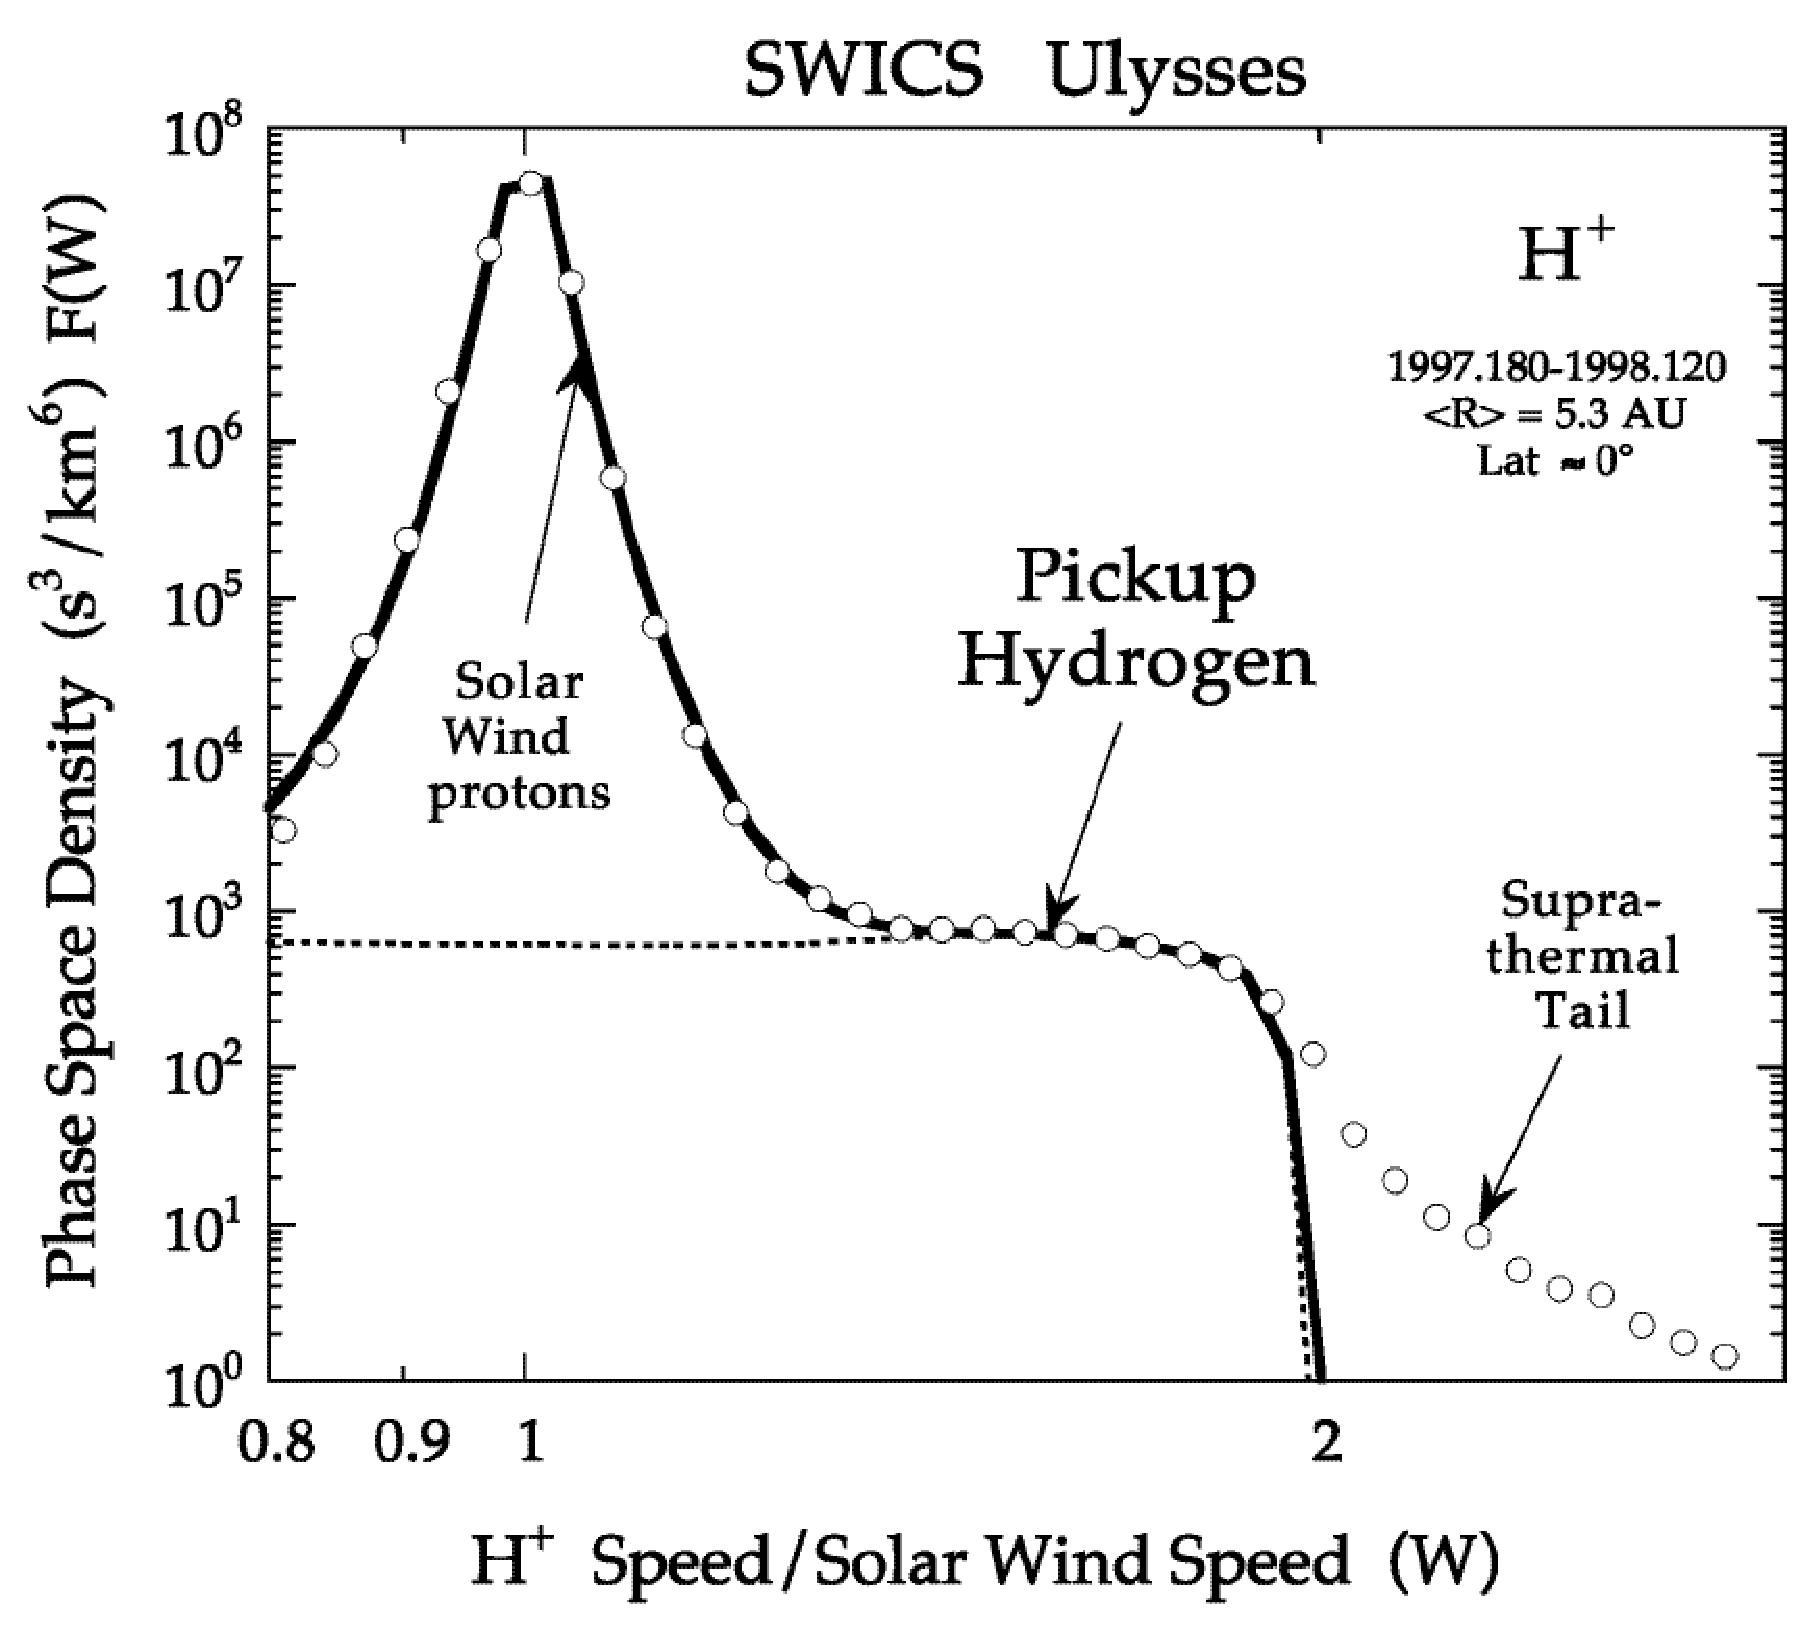
\includegraphics[width=.65\textwidth]{format/H_Distribution}
  \caption[Example of proton distributions for the quiet solar wind near 5 AU.]{Example of proton distributions for the quiet solar wind near 5 AU. Shown are the bulk distribution of the solar wind, the interstellar pickup ions that drop off at twice the solar wind speed, and the high-energy protons that make up the suprathermal tail. Figure from \citet{gloeckler01b}.}
  \label{fig:H_Distribution}
\end{figure}

\section{The Solar Wind}
\label{Solar Wind}

\subsection{Current Knowledge}
\label{SW Current Knowledge}
While he was not the first to postulate its existence, the physics of the solar wind was first explained by Eugene Parker in 1958 \citep{parker58}. Beginning with subsonic speeds close to the Sun, plasma accelerates away from the solar surface and reaches supersonic speeds in the corona. It continues to expand in a radial direction outward until it interacts with the material in interstellar space at the edge of the heliosphere, the Sun's sphere of influence. The wind draws the solar magnetic field along with it, creating spiral-shaped field lines as the Sun rotates \citep{parker59}. Mankind's understanding of the processes that govern the solar wind has increased as spacecraft have taken in situ measurements, but there are still some properties that remain unexplained, such as the precise origin of certain types of wind, as discussed below.

The solar wind travels a distance of one \ac{AU} before reaching Earth's orbit, where most of the current measurements have been taken (Table~\ref{tab:solar wind}). It is generally divided into two components, commonly referred to as the ``fast'' and ``slow'' solar wind. Originally, these terms were used to differentiate the wind by the speed with which it traveled, but more recent studies have shown that the two types of wind are more efficiently distinguished by their charge state composition (e.g., O$^{7+}$/O$^{6+}$) since the plasma can change speeds as it flows through space \citep{geiss95b, gloeckler03a}. Rather than the terms ``fast'' and ``slow'', more appropriate labels are descriptive of the wind's origin: ``coronal hole'' and ``streamer'' wind. These two types of wind are generated by different processes and have different compositions, temperatures, speeds, and origins.
\begin{table}[htbp]
	\centering
		\begin{tabular}{l|c|c}
		                                                               & Coronal Hole Wind & Streamer Wind     \\ \hline
      bulk speed \footnotesize{$\left(\text{km s}^{-1}\right)$}    & 750               & 400               \\ \hline
      thermal speed \footnotesize{$\left(\text{km s}^{-1}\right)$} & 32                & 35                \\ \hline
      H$^+$ density \footnotesize{$\left(\text{cm}^{-3}\right)$}   & 2.5               & 8.7               \\ \hline
      frozen-in temperature \footnotesize{$\left(\text{K}\right)$} & 8 x 10$^5$        & 1.4--1.6 x 10$^6$ \\ \hline

		\end{tabular}
	\caption[Average characteristics of the solar wind at 1 AU.]{Average characteristics of the solar wind at 1 AU. The temperature is derived from the freeze-in temperature of C$^{6+}$/C$^{5+}$, which freezes in near the solar wind source altitude. Data compiled from \citet{vonsteiger95, gloeckler98a, ipavich98, mccomas00, feldman05}.}
	\label{tab:solar wind}
\end{table}

As solar wind ions escape from the photosphere and travel up through the corona, they experience collisions with energetic electrons that ionize them to different degrees. As they travel farther through the corona, continuously accelerating, the density of coronal electrons decreases and the particles experience fewer collisions. When the timescale for ionization or recombination becomes longer than the timescale of the solar wind to expand through a density scale height, the charge state of the ion is said to be ``frozen in,'' branding the ion with the coronal region and electron temperature of its origin \citep{hundhausen68}. The streamer wind has a distinct characteristic of being enriched in elements with a low ($\le$ 10 eV) \ac{FIP} by a factor of 3--4 over the photospheric value. The coronal hole wind does not show this density enhancement, and measurements have revealed abundances of low-\ac{FIP} elements that match ratios in the photosphere \citep{vonsteiger93}. The streamer wind also has a higher and more variable freeze-in temperature than the coronal hole wind. One explanation for this describes solar plasma trapped and heated in large coronal loops that are eventually opened by interchange reconnection, releasing the plasma \citep{gosling95, fisk98, fisk99a}.

The coronal hole wind originates in the open flux regions of the Sun, which contain low-density plasma and concentrations of magnetic flux that are all the same polarity. During solar minimum these regions are clustered around the poles of the Sun, while during solar maximum they appear at all latitudes. Plasma in open flux regions is also released from flux loops, but the high concentration of open flux increases the probability that the loops will open before they can heat and fractionate the plasma. The anti-correlation between freeze-in temperature and solar wind speed shown in Table~\ref{tab:solar wind} can be interpreted in a simplistic way as a sign of different sized loops. The long-lived loops that produce the streamer wind will expand and rise slowly into the corona, where the temperatures are hotter, before being opened \citep{fisk98, fisk01a}. The short-lived loops that yield the coronal hole wind are opened while they are still small and close to the cooler surface \citep{fisk99a, fisk03, wimmer03b}.

 \chapter{Electronic Mechanism of H adsorptions on ZnO Surfaces}
 \label{chap:ZnO_H}
 \input{Chap1/chap1}
 
 \chapter{Alloy segregations in Ag grain boundaries}
 \label{chap:Ag_W}
 \input{Chap2/chap2}
 
 \chapter{Using alloy to enhance corrosion resistance of Mg alloy with transition metal impurities}
 \label{chap:Mg_H}
 \input{Chap3/chap3}
 
 \chapter{Grand Canonical Monte Carlo simulations of Ag thin film depositions}
 \label{chap:Ag/ZnO}
 \input{Chap4/chap4}
 
 \chapter{Kinetic Monte Carlo simulations of Solute Clustering in multi-component Al alloys}
 \label{chap:Al/Vac}
 \input{Chap5/chap5}
 
 \chapter{Summary and Future Work}
 \label{chap:Conc}
 \section{Summary}

\section{Future Work}
 
\startappendices
 \appendix{Passivation of Zn-terminated ZnO (0001) Surface}
 \label{appd:passivation}
 
As mentioned in Sec. \ref{sec:Hcoverage}, the above coverage-dependent H adsorption strengths $E_{\textup{ad}}^{\textup{H}}$ on O-terminated (000$\overline{1}$) ZnO surface may change due to different passivation methods on the Zn-terminated (0001) surface, where each Zn atom has a dangling bond with 0.5 unpaired electron in its bulk-terminated ideal form. The dangling bond of each surface Zn atom should be emptied to reach the passivated structure and eliminate the artificial charge transfer from (0001) to (000$\overline{1}$) surface according to the classical electron counting model\cite{pashley1989electron}. It can be achieved by generating a  $\frac{1}{4}$ ML Zn vacancy on (0001) surface layer (one Zn vacancy in the (2$\times$2) supercell) because the 0.5 unpaired electron from each of 3 remaining Zn atoms on (0001) surface can transfer to each of 3 O atoms that are the first-nearest neighbors of the Zn vacancy to form the stable closed-shell electron configurations. In addition, the passivated (0001) surface can also be achieved by adding one atom, such as a pseudo-hydrogen atom with 1.5 electrons (H$_{1.5}$), to each Zn atom on (0001) surface to fill the dangling bond.

\begin{table}[!htbp]
\centering
\caption[Comparison of different passivation mechanisms for the coverage-dependent adsorption energy of H atom]{The coverage-dependent adsorption energy of H atom $E_{\textup{ad}}^{\textup{H}}$ in unit of eV on (2$\times$2) O-terminated (000$\bar{1}$) ZnO surface with different mechanisms to passivate the Zn-terminated (0001) surface, including a clean Zn-terminated surface, a $\frac{1}{4}$ ML Zn vacancy (V$_{\textup{Zn}}$) on the Zn-terminated surface and pseudo-hydrogen atoms with different numbers of valence charges (1.5, 1.0 and 0.5 electron, respectively) at each Zn site on the Zn-terminated surface (H$_{1.5}$, H$_{1.0}$ and H$_{0.5}$).}
\label{tab:pass}
\begin{tabular}{lllll}
\hline
\hline
eV/Atom       & 0.25ML & 0.5ML & 0.75ML & 1ML  \\ \hline
V$_{\textup{Zn}}$     & -2.43  & -2.18 & 0.43   & 0.95 \\
H$_{1.5}$         & -2.45  & -2.28 & 0.42   & 0.96 \\
H$_{1.0}$         & -2.45  & -2.27 & 0.11   & 0.95 \\
H$_{0.5}$         & -2.38  & -1.82 & 0.43   & 0.98 \\ 
Clean Zn-terminated & -2.34  & -1.49 & 0.52   & 0.95 \\
\hline
\hline
\end{tabular}
\end{table}

Tab.\ref{tab:pass} lists the H adsorption energies on (2$\times$2) (000$\overline{1}$) ZnO calculated using different passivation methods: the addition of Zn vacancies or (pseudo-)hydrogen atoms with different numbers of valence charges (H$_{1.5}$, H$_{1.0}$, and H$_{0.5}$) on (0001) surface. 
$\frac{1}{4}$ ML Zn vacancy (V$_{\textup{Zn}}$) and H$_{1.5}$ generate almost the same $E_{\textup{ad}}^{\textup{H}}$ on (000$\bar{1}$) for all investigated H surface coverages $\theta_{\textup{H}}$. These results confirm that both methods can fully passivated the Zn-terminated surface and eliminate the artificial electron transfer in the supercell. Meanwhile, an obvious difference between  H$_{1.0}$ and H$_{1.5}$ cases can be observed for the adsorption of the third H atom in the (2$\times$2) supercell ($\theta_{\textup{H}}$ = $0.75$ ML), where $E_{\textup{ad}}$ of H$_{1.0}$ case is 0.11 eV, $\sim$ 0.3eV lower than the values for V$_{\textup{Zn}}$ and H$_{1.5}$ cases. This is because one H$_{1.0}$ atom cannot completely fully filled the bonding bond of each Zn atom on (0001). For the cases of Zn-terminated surfaces without pseudo-hydrogen atoms (Clean Zn-terminated in Tab. \ref{tab:pass}) and the cases of H$_{0.5}$, because there are large amounts of electron transfers from Zn-terminated to O-terminated surfaces, H adsorption energies on the O-terminated surfaces are much weaker than those of V$_{\textup{Zn}}$ and H$_{1.5}$ cases for $\theta_{\textup{H}}$ = $0.5$ and $0.75$ ML. Thus, in the paper, only the results corresponding to H$_{1.5}$ cases (fully passivated Zn-terminated surfaces) are reported.
 
\startbibliography
 \begin{singlespace} % Bibliography must be single spaced
  \bibliography{References}   % Use the BibTeX file ``References.bib''.
 \end{singlespace}

% An external Abstract that can be printed at the end of the document, 
% for separate submission to Rackham. Comment it out when not needed. - jg
%\startextabstractpage
%{The Title of Your Dissertation}{Your Name}{Chair: Albert Einstein}
%In my dissertation, the thermodynamic driving forces and kinetics of critical reaction steps during advanced alloy processing are studied systematically by theoretical models and simulation tools at the atomistic scale. These efforts include improving the Ag thin-film quality during sputtering, discovering a build-in corrosion-resistant mechanism for cast Mg alloys, and slowing down cluster nucleation and growth in Al solid solution alloys during natural aging to avoid costly hot stamping procedures. First, the thermodynamic driving force of H adsorption on anion-terminated (000$\overline{1}$) surfaces of pure and doped wurtzite ZnO as dielectric substrates are investigated under varying H surface coverage conditions. Understanding of these H adsorption mechanisms provides a general way to design substrate surfaces with desired binding strengths for the Ag thin-film. Second, \acf{GCMC} simulations are conducted to simulate the deposition "kinetics" of Ag thin film on substrates, which can be constructed based on the structures and properties of H-adsorbed ZnO (000$\overline{1}$) surfaces. The results demonstrate the reason why ZnO is the most suitable substrate for Ag thin film deposition and the mechanism to achieve thinner continuous Ag films by adding "anchor'' sites on the substrate surface. We use first-principles calculations to search for potential dopant elements as good "anchor'' sites on ZnO substrates and other dopants to stabilize the Ag grain boundaries to improve the polycrystalline Ag thin-film during heat treatment. Third, the \acf{HER} as the cathodic reaction on surfaces of the second-phase transition-metal (Fe) particles can speed up the corrosion of cast Mg metals and alloy. Thus, thermodynamic criteria to slow down the HER are used for high-throughput first-principles computations to search alloying elements that can reduce HER rate to achieve build-in corrosion resistance for cast Mg alloys. Our first-principles search goes across the periodic table and discovers six p-block elements that can increase the corrosion resistance for Mg, consistent with the available experimental results. Fourth, \acf{kMC} simulations are performed to study the early transition behavior from a supersaturated solid solution to \acf{GP} zone of Al 7000 series alloys at room temperature (so-called natural aging), which is critical for their thermal-mechanical processing in automobile manufacturing. Our kMC method include a \acf{NN} model trained by thousands of \ac{DFT} calculations to accurately predict vacancy migration barriers in Al-Mg-Zn-based alloys. Besides, advanced modeling approaches like \acf{LRU} cache and \acf{LSKMC} are also implemented to speed up the kMC simulations in order to directly study the natural aging of Al alloys in the realistic time scales.
%\label{ExtAbstract}

\end{document}